The likelihood ratio LRhas been evaluated for six different values of $m_H$ between 250 and 600 \GeVcc.
Figure~\ref{fig:lrstacksHZZ} shows the likelihood ratio distributions for $m_H$~=~250, 300, 400, and 500 \GeVcc,               
corresponding to 4.7~fb$^{-1}$.

\begin{figure}[!hbtp]                                                                                         
\centering                                                                                                    
\subfigure[]{                                                                                                 
\centering                                                                                                    
\label{subfig:lr_hm250HZZ}                                                                                       
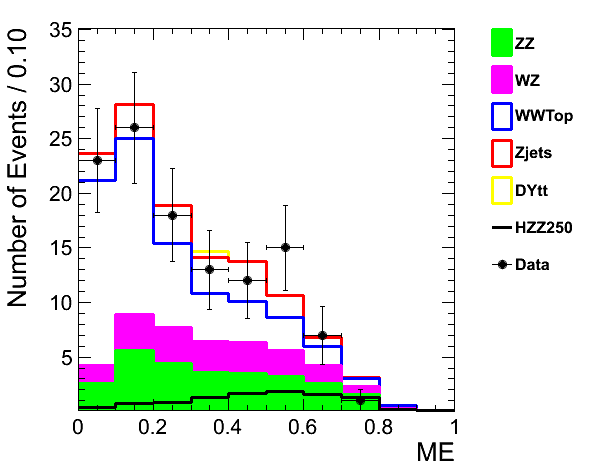
\includegraphics[width=.40\textwidth]{figures/ME_mH250_ee_stack_lin.png}                                                 
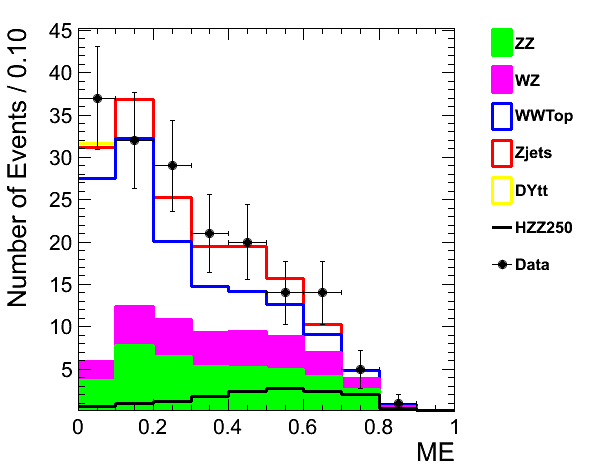
\includegraphics[width=.40\textwidth]{figures/ME_mH250_mm_stack_lin.png}}                                                 
\subfigure[]{                                                                                                 
\centering                                                                                                    
\label{subfig:lr_hm300HZZ}                                                                                       
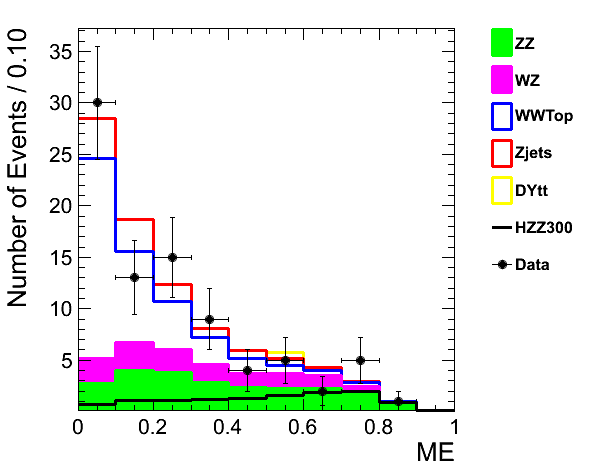
\includegraphics[width=.40\textwidth]{figures/ME_mH300_ee_stack_lin.png}                                                 
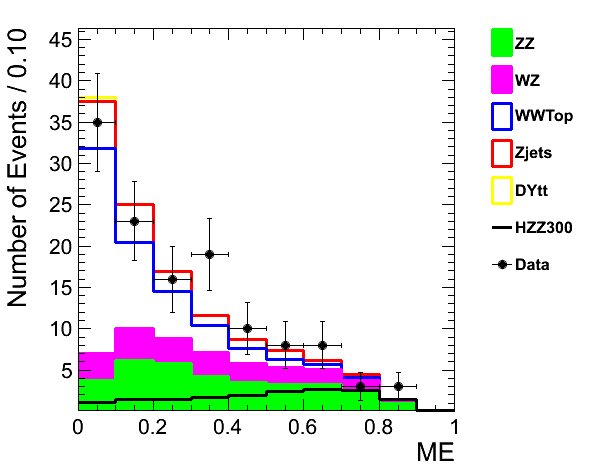
\includegraphics[width=.40\textwidth]{figures/ME_mH300_mm_stack_lin.png}}                                                 
\subfigure[]{                                                                                                 
\centering                                                                                                    
\label{subfig:lr_hm400HZZ}                                                                                      
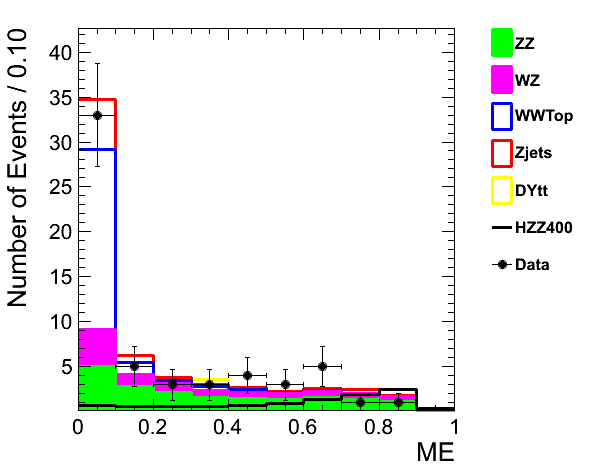
\includegraphics[width=.40\textwidth]{figures/ME_mH400_ee_stack_lin.png}                                                 
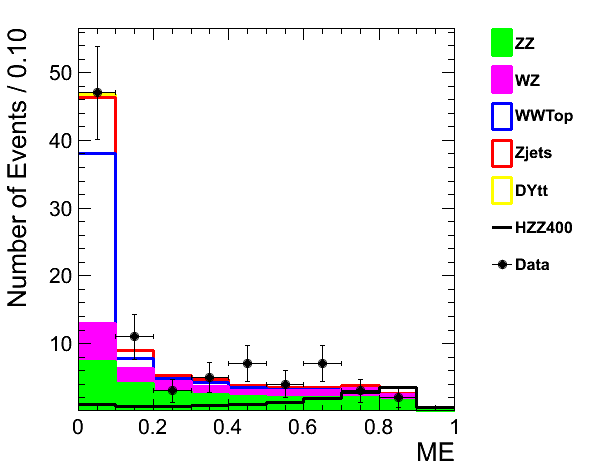
\includegraphics[width=.40\textwidth]{figures/ME_mH400_mm_stack_lin.png}}                                                 
\subfigure[]{                                                                                                 
\centering                                                                                                    
\label{subfig:lr_hm500HZZ}                                                                                       
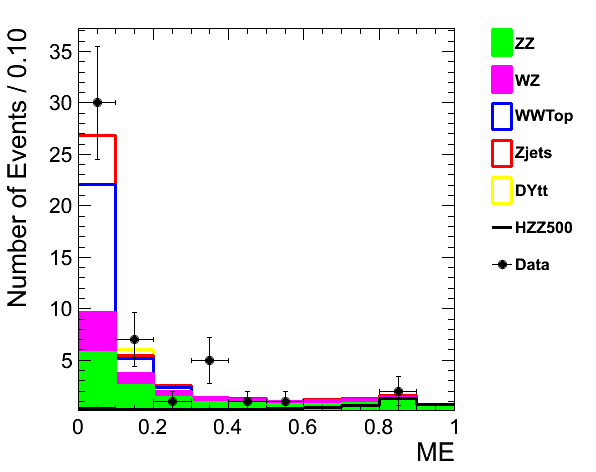
\includegraphics[width=.40\textwidth]{figures/ME_mH500_ee_stack_lin.png}                                                 
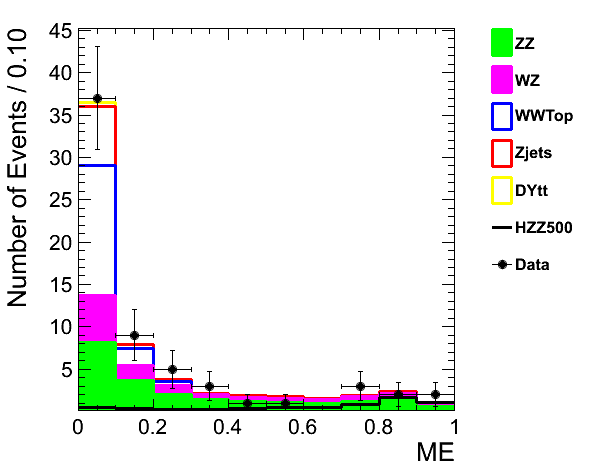
\includegraphics[width=.40\textwidth]{figures/ME_mH500_mm_stack_lin.png}}\\                                                 
\caption{The matrix element based Likelihood Ratio distribution after event selection,                     
for $m_H$=250 \GeVcc \subref{subfig:lr_hm250HZZ}, $m_H$=300 \GeVcc \subref{subfig:lr_hm300HZZ}, $m_H$=400 \GeVcc 
\subref{subfig:lr_hm400HZZ}, and $m_H$=500 \GeVcc \subref{subfig:lr_hm500HZZ} in the 0-jet bin, shown separately for $ee$ (left)
and $\mu\mu$ (right) events.}                                            
\label{fig:lrstacksHZZ}                                                                                          
\end{figure}            

We compute the upper limit using the shape of the LR distribution. 
The expected and observed asymptotic CLs upper limits at 95\% C.L from the matrix element based method is shown in 
Figure~\ref{fig:me_expected_1.1fb_HZZ} as a function of $m_H$
and tabulated in Table~\ref{tab:me_expected_1.1fb_HZZ}.  The same figure and table show the upper limits obtained using 
the cut-based and $m_{T}$ shape based approaches from \cite{ref:HZZ2011smurf}. The comparison reveals that use of the Matrix Element 
technique provides a substantial 15-25$\%$ improvement in the sensitivity when compared to the cut-based analysis. When compared
to $m_{T}$ shape based results, ME performs 10\% better at lower $m_{H}=250--300$ \GeVcc and equally well at higher masses.

\begin{figure}[!hbtp]
\centering
\subfigure[]{
\label{subfig:limit_MEshape}
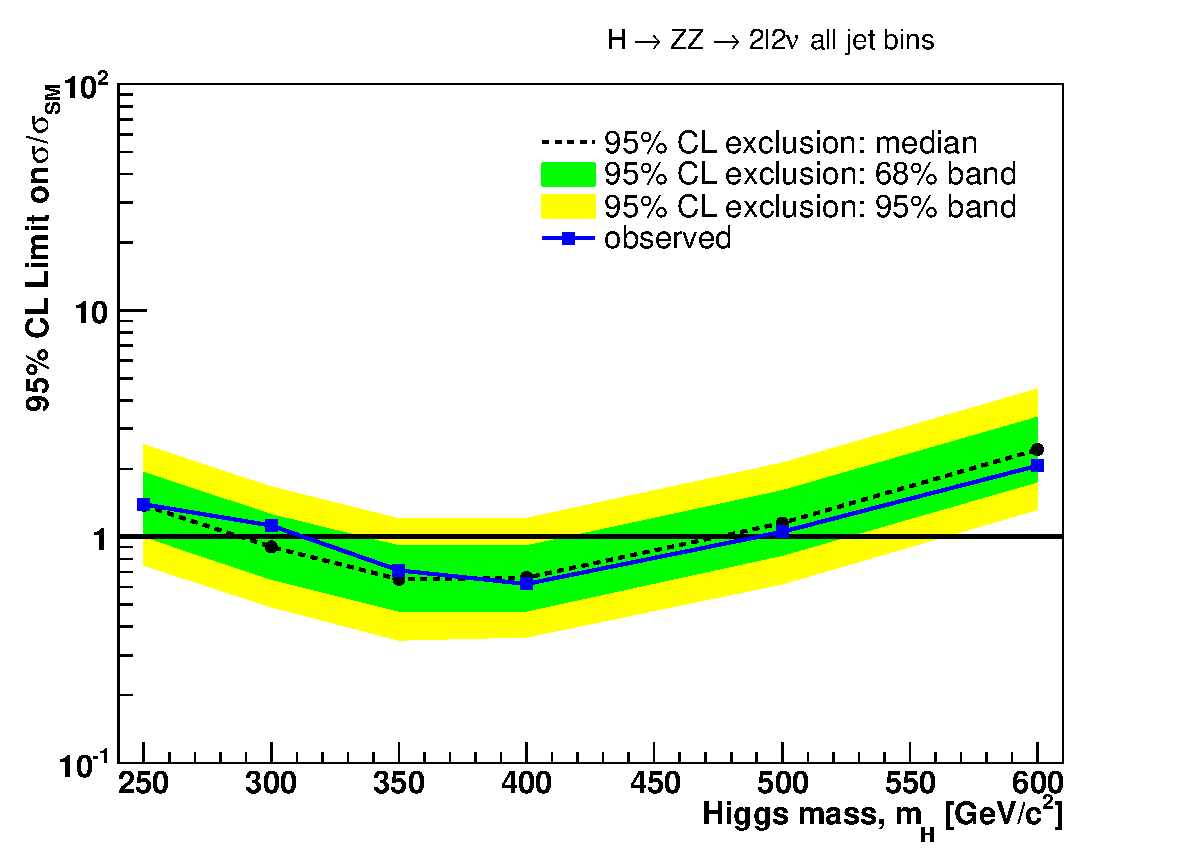
\includegraphics[width=.5\textwidth]{figures/limits_me_4700pb_shapesyst.pdf}}
\subfigure[]{
\label{subfig:limit_mtshape}
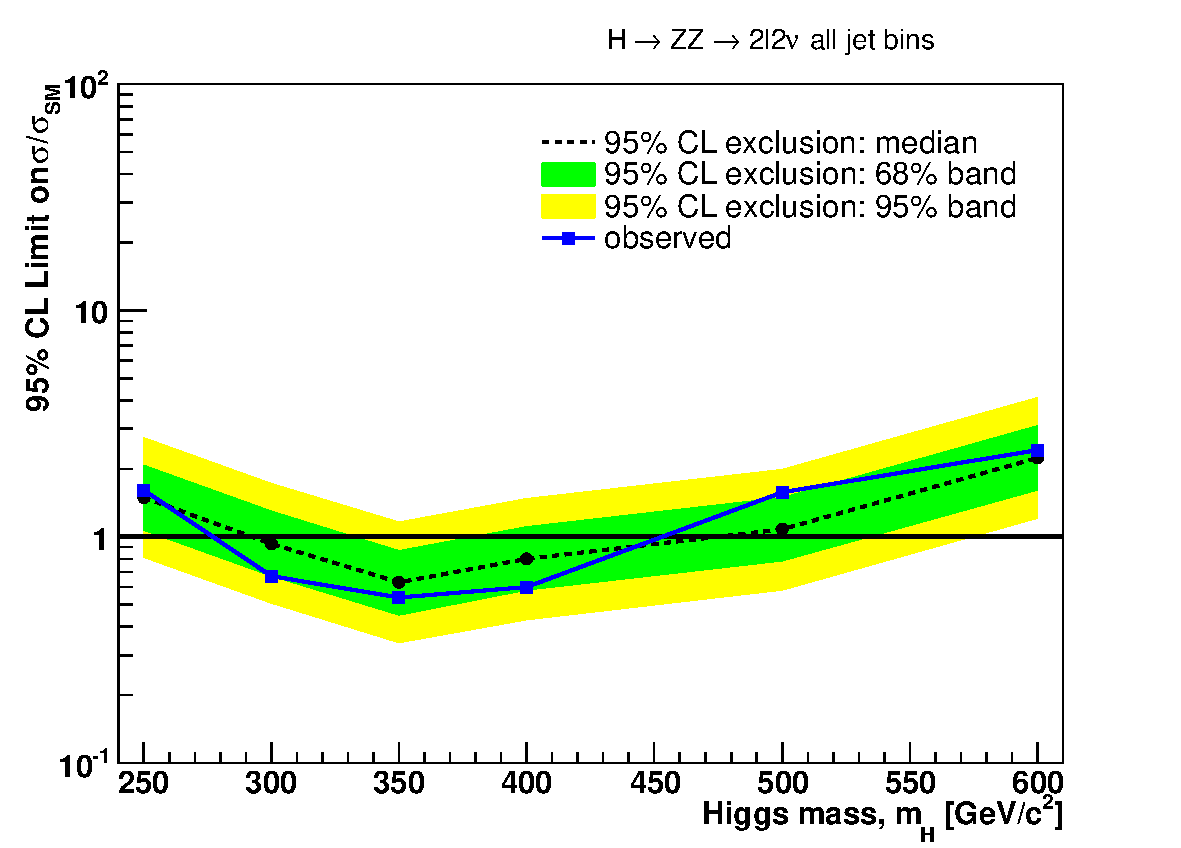
\includegraphics[width=.5\textwidth]{figures/limits_mt_4700pb_shapesyst.pdf}}
\subfigure[]{
\label{subfig:limit_cuts}
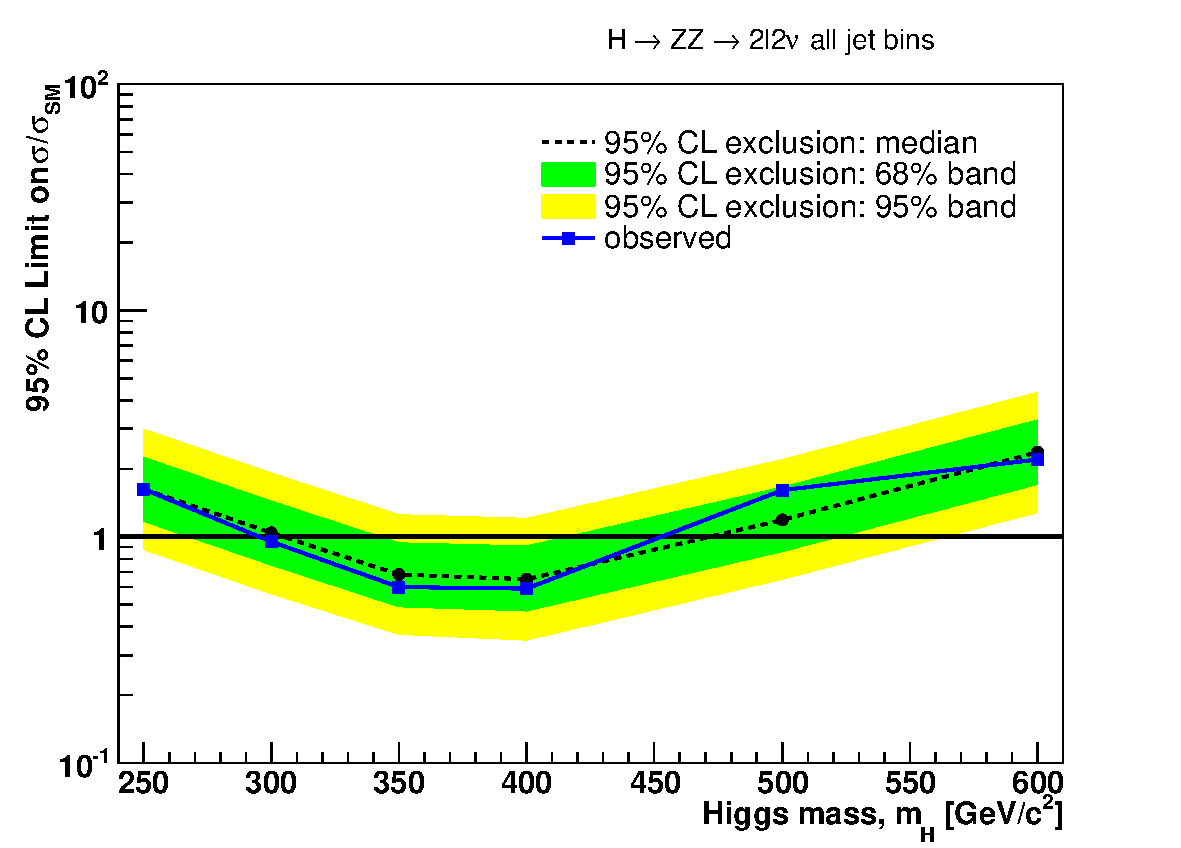
\includegraphics[width=.5\textwidth]{figures/limits_cut.pdf}}
\caption{ 
Expected and observed asymptotic CLs upper limits at 95\% C.L. for 4.7~fb$^{-1}$ data using the 
matrix elemement \subref{subfig:limit_MEshape}, transverse mass shape \subref{subfig:limit_mtshape},
and cut-based approach \subref{subfig:limit_cuts}. } 
\label{fig:me_expected_1.1fb_HZZ}
\end{figure}


%%%%%%%%%%%%%%%%%%%%%%%%%%%%%%
\begin{table}
\begin{center}
\begin{tabular}{ccccc}
\hline
\multicolumn{4}{c} {Matrix Element Method} \\
\hline
Mass & Observed & Median Expected & [-$\sigma$, +$\sigma$] & [-2$\sigma$, +2$\sigma$]\\\hline
250 & 1.39 & 1.38 & [1.00, 1.92] & [0.75, 2.55] \\
300 & 1.12 & 0.90 & [0.65, 1.25] & [0.49, 1.66] \\
350 & 0.71 & 0.65 & [0.47, 0.91] & [0.35, 1.20] \\
400 & 0.62 & 0.66 & [0.47, 0.91] & [0.36, 1.21] \\
500 & 1.05 & 1.15 & [0.83, 1.60] & [0.62, 2.12] \\
600 & 2.06 & 2.43 & [1.75, 3.37] & [1.32, 4.48] \\
\hline
\multicolumn{4}{c} {$m_{T}$-based Method} \\
\hline
250 & 1.61 & 1.49 & [1.07, 2.07] & [0.81, 2.75] \\
300 & 0.67 & 0.93 & [0.67, 1.30] & [0.51, 1.72] \\
350 & 0.54 & 0.63 & [0.45, 0.87] & [0.34, 1.16] \\
400 & 0.60 & 0.80 & [0.58, 1.11] & [0.43, 1.48] \\
500 & 1.57 & 1.08 & [0.78, 1.49] & [0.58, 1.99] \\
600 & 2.42 & 2.23 & [1.61, 3.10] & [1.21, 4.12] \\
\hline
\multicolumn{4}{c} {Cut-and-count based Method} \\
\hline
250 & 1.62 & 1.62 & [1.17, 2.24] & [0.88, 2.98] \\
300 & 0.95 & 1.04 & [0.75, 1.44] & [0.56, 1.91] \\
350 & 0.60 & 0.68 & [0.49, 0.94] & [0.37, 1.25] \\
400 & 0.59 & 0.65 & [0.47, 0.91] & [0.35, 1.21] \\
500 & 1.61 & 1.19 & [0.86, 1.66] & [0.65, 2.20] \\
600 & 2.20 & 2.36 & [1.70, 3.28] & [1.28, 4.36] \\
\hline    
\end{tabular}
\end{center}
\caption{Expected asymptotic CLs upper limits at 95$\%$ C.L. for 4.7~fb$^{-1}$ data using the 
matrix elemement output corresponding to Figure~\ref{fig:me_expected_1.1fb_HZZ}. Upper limits
obtained using cut-based method are also given for comparison.}
\label{tab:me_expected_1.1fb_HZZ}
\end{table}